\chapter{Guía de solución de problemas}
\label{chapter: troubleshooting}

\section{Mensajes de error}
Existen dos mensajes de error que la interfaz gráfica arrojará
al usuario de acuerdo a los datos que el usuario introduzca.
Ambos mensajes están diseñados para informar al usuario que
la posición deseada no es alcanzable con las condiciones provistas
al sistema.
El sistema arrojará un mensaje de acuerdo al valor conflictivo.
Para solucionar ambos errores, actualice la posición deseada 
o los valores de la plataforma para permitir al simulador
encontrar una solución válida.

\begin{itemize}
 \item \textbf{Aviso de hiper-extensión}. El robot es incapaz 
 de alcanzar la \emph{posición} deseada ya que está fuera del alcance 
 del mismo. 
%  Ejemplo: un robot cuya máximo desplazamiento en 
%  el eje z sea 1 metro será incapaz de alcanzar una posición 
%  de 5 metros.
 
 \begin{figure}[h]
 \centering
 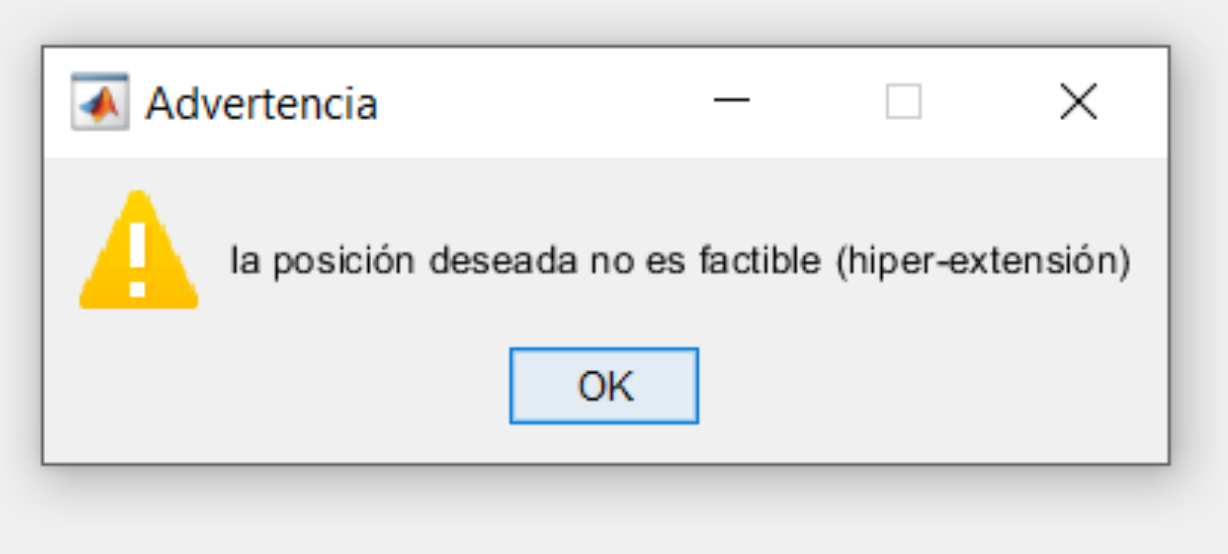
\includegraphics[scale=0.3]{img/hiperextension.png}
 % hiperextension.png: 1228x554 px, 96dpi, 32.49x14.66 cm, bb=0 0 921 415
 \caption{Error de hiper-extensión.}
 \label{fig: hyper-extension}
\end{figure}

 
  \item \textbf{Aviso de hiper-compresión}. El robot es incapaz 
 de alcanzar la \emph{orientación} deseada ya que la compresión
 de los pistones limita el reacomodo de la plataforma superior.
 \end{itemize}
  
 \begin{figure}[h]
 \centering
 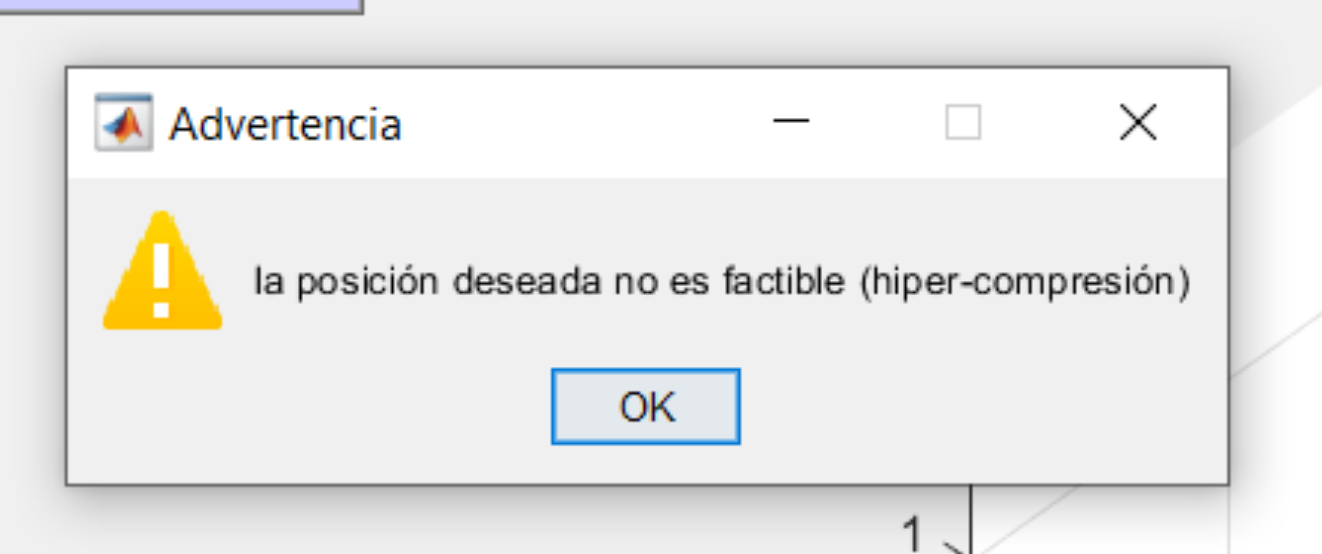
\includegraphics[scale=0.3]{img/hipercompresion.png}
 % hiperextension.png: 1228x554 px, 96dpi, 32.49x14.66 cm, bb=0 0 921 415
 \caption{Error de hiper-compresión.}
 \label{fig: hyper-compresion}
\end{figure}
